\documentclass{article}
\usepackage{qilin}
\tikzstyle{process} = [rectangle, rounded corners, minimum width=1.5cm, minimum height=0.5cm,align=center, draw=black, fill=gray!30, auto]
\title{PHY294: Practice Problems \\ \textbf{Problem Set 2 Solutions}}
\author{QiLin Xue}
\date{Winter 2022}
\usepackage{mathrsfs}
\usetikzlibrary{arrows}
\usepackage{siunitx}
\begin{document}

\maketitle
\begin{enumerate}[label=(9.\arabic*)]
    \setcounter{enumi}{0}
    \item The magnitude is $S=\sqrt{s(s+1)}\hbar=\sqrt{3}/2\hbar$ where $s=1/2$ for an electron, and $S_z = \pm \frac{1}{2}\hbar.$ Therefore, the angle between $\vec{S}$ and $e_z$ is 
        \begin{equation}
            \theta = \arccos\frac{S_z}{S} = 54.736^\circ.
        \end{equation}
    \setcounter{enumi}{2}
    \item \begin{enumerate}
        \item We have $S_z = m_s\hbar{h}$ where $m_s\in\{1,0,-1\}$. Therefore, it can take on three possible values.
        \item Angle can be calculated using same method as previous question.
        \item The minimum possible angle is when $S_z$ is closest to $S$, i.e. when $m_s = 1.$ This gives 
        \begin{equation}
            \theta_\text{min} = 45^\circ.
        \end{equation}
    \end{enumerate}
    \setcounter{enumi}{4}
    \item This corresponds to the $1s^22s^22p^6$ state.
    \begin{itemize}
        \item For $(n,\ell) = (1,0)$, we have $m=0$, so there are two possible values for $m_s$.
        \item For $(n,\ell) = (2,0)$, we have $m=0$, so there are two possible values for $m_s$.
        \item For $(n,\ell) = (2,1)$, we have $m\in\{-1,0,1\}$, so there are six possible values for $m_s$.
    \end{itemize}
    \setcounter{enumi}{7}
    \item The moment of inertia of a ball is $I \approx mr^2$ (Note that the distribution of mass may change this, possibly by a factor of $\frac{2}{5}$, but it's the order of magnitude that counts). The angular momentum is then:
    \begin{equation}
        mr^2\frac{v}{r} \sim \hbar \implies \frac{v}{c} \sim \frac{\hbar}{mrc} \approx 40,000,
    \end{equation}
    which clearly isn't possible!
    \item \begin{enumerate}
        \item The magnetic moment is $\mu = I(\pi r^2) = 1.26 \times 10^{-4} \si{\ampere\meter\squared}$
        \item The torque is $\tau = \mu B \sin\theta = 1.89\times 10^{-4} \si{\ampere\meter\squared\tesla}.$
        \item The potential energy is $U = -\mu B\cos\theta.$ If $B$ is flipped, then $\cos\theta$ goes from $1$ to $-1$, and therefore $\Delta U = -2\mu B = -3.78\times 10^{-4} \si{\joule}.$
    \end{enumerate}
    \setcounter{enumi}{10}
    \item Similar to above, we have $\mu = I(\pi r^2) \implies I = \frac{\pi r^2}{\mu} = 3.18\times 10^{-4}\si{\ampere}.$
    \setcounter{enumi}{14}
    \item \begin{enumerate}
        \item See below
        \begin{center}
            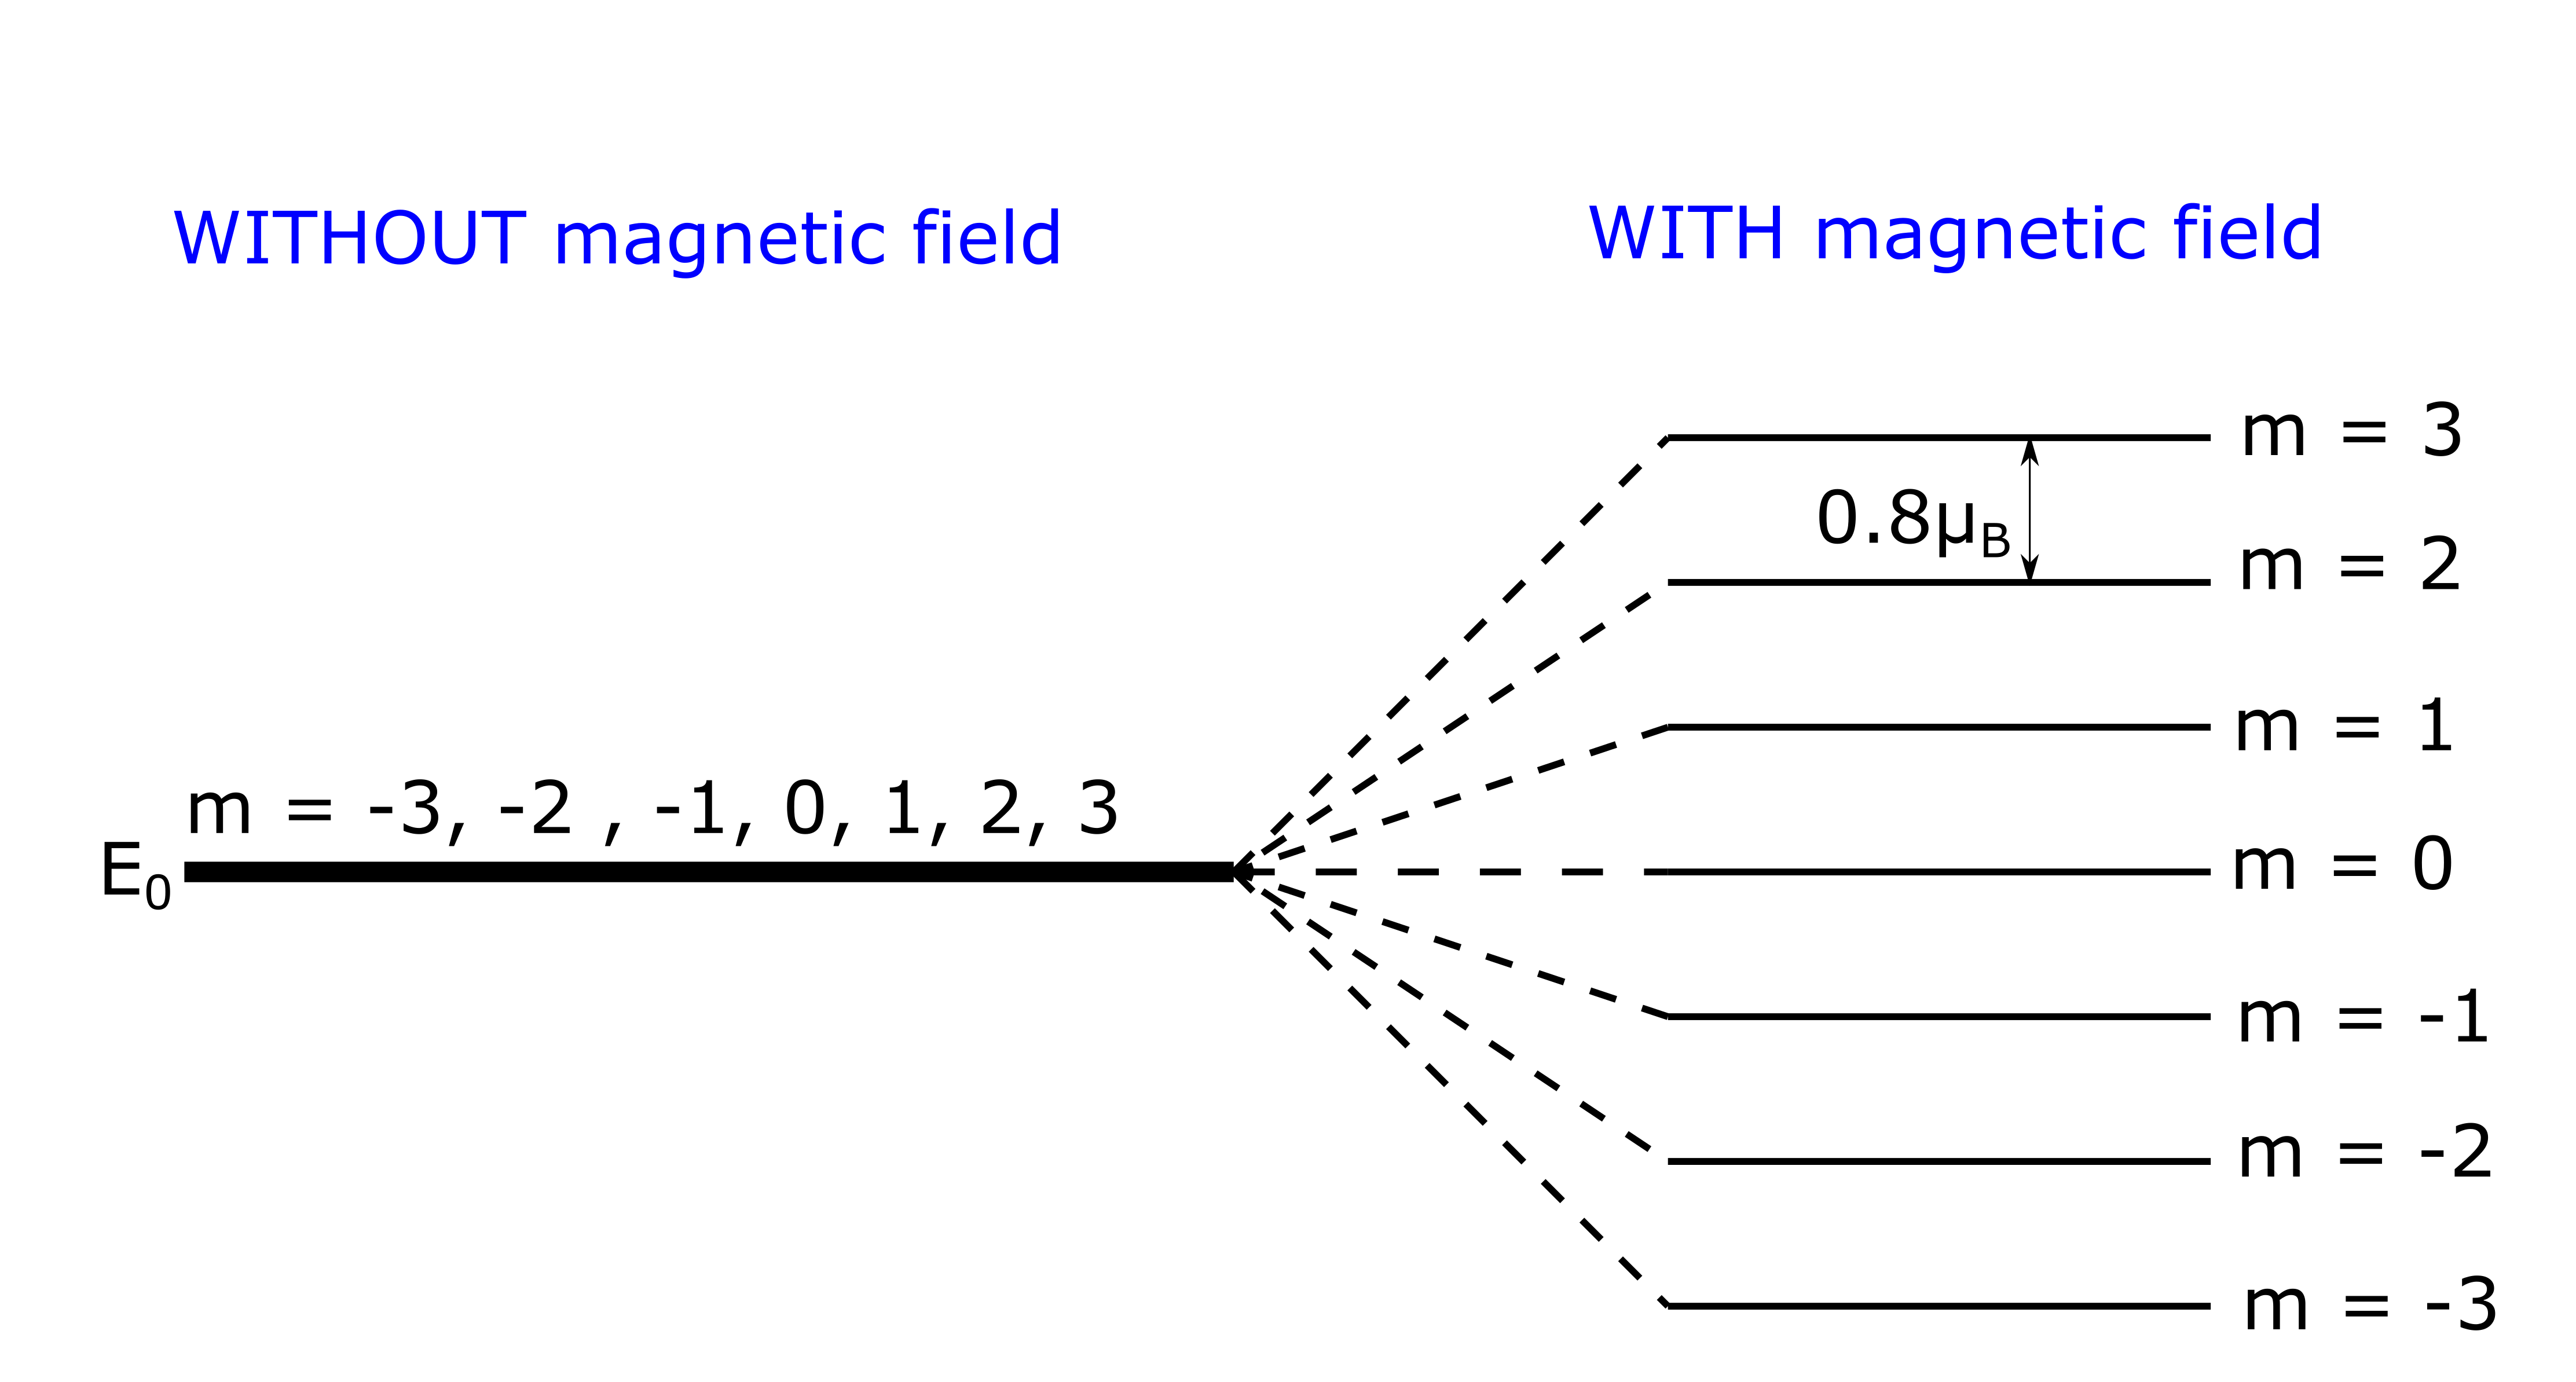
\includegraphics[width=0.7\linewidth]{figs/9.15.png}
        \end{center}
        \item The energy difference between adjacent levels is $\mu_B B$, where $\mu_B=9.27\times 10^{-24} \si{\joule\per\tesla}$ is the Bohr magneton.
    \end{enumerate}
    \setcounter{enumi}{16}
    \item \begin{enumerate}
        \item Very similar to the above diagram except in the higher level there are $2l+1=5$ sub-levels while in the lower level there are $2l+1=3$ sub-levels.
        \item Since $\Delta E \propto L_z$, which is dependent on $m_i,m_f$, let us look at the number of distinct differences $m_f-m_i$ (now this is just a statistics problem!) If $m_i=1$, there are five possible differences. If $m_i=0$, there are still five possible differences, but only one of them will be new. The same goes for $m_i=-1$. Therefore, there are $5+1+1=7$ possible photon energies.
        \item To see why this is true, note that
        \begin{align*}
            E_f &= E_{0,f} + \mu_B B m_f \\ 
            E_i &= E_{0,i} + \mu_B Bm_i
        \end{align*}
        and so
        \begin{equation}
            E_\gamma = E_f - E_i = (E_{0,f}-E_{0,i}) + \mu_BB(m_f-m_i).
        \end{equation}
        The photon energy is dependent on $m_f-m_i.$ Since this can only take on three values, the photon energy can only take on three values.
    \end{enumerate}
    \setcounter{enumi}{18}
    \item \begin{enumerate}
        \item For the anomalous Zeeman effect, we have
        \begin{equation}
            E_\text{diff} = 2\mu_BB = 1.3\times 10^{-23}\si{\joule}
        \end{equation}
        \item Using the relationship $E_\gamma\lambda = hc$, we determine the wavelength to be on the order of magnitude of $1\text{ cm}$, which corresponds to microwaves.
    \end{enumerate}
\end{enumerate}
\end{document}